\documentclass[10pt]{article}
\usepackage[margin=1in]{geometry} 
\usepackage{fancyhdr}
\pagestyle{fancy}
\usepackage{amsmath,amsthm,amssymb}
\usepackage{float}
\usepackage[pdftex]{graphicx}
\usepackage{color}
\usepackage{mathtools}          %loads amsmath as well
\usepackage{mdframed}
\DeclarePairedDelimiter\Floor\lfloor\rfloor
\DeclarePairedDelimiter\Ceil\lceil\rceil
 
\newcommand{\N}{\mathbb{N}}
\newcommand{\Z}{\mathbb{Z}}
 
\newenvironment{theorem}[2][Theorem]{\begin{trivlist}
\item[\hskip \labelsep {\bfseries #1}\hskip \labelsep {\bfseries #2.}]}{\end{trivlist}}
\newenvironment{lemma}[2][Lemma]{\begin{trivlist}
\item[\hskip \labelsep {\bfseries #1}\hskip \labelsep {\bfseries #2.}]}{\end{trivlist}}
\newenvironment{exercise}[2][Exercise]{\begin{trivlist}
\item[\hskip \labelsep {\bfseries #1}\hskip \labelsep {\bfseries #2.}]}{\end{trivlist}}
\newenvironment{problem}[2][Problem]{\begin{trivlist}
\item[\hskip \labelsep {\bfseries #1}\hskip \labelsep {\bfseries #2.}]}{\end{trivlist}}
\newenvironment{question}[2][Question]{\begin{trivlist}
\item[\hskip \labelsep {\bfseries #1}\hskip \labelsep {\bfseries #2.}]}{\end{trivlist}}
\newenvironment{corollary}[2][Corollary]{\begin{trivlist}
\item[\hskip \labelsep {\bfseries #1}\hskip \labelsep {\bfseries #2.}]}{\end{trivlist}}

\newenvironment{solution}{\begin{proof}[Solution]}{\end{proof}}

 
\begin{document}
 
\lhead{ECE 527 - MP4 Lenet}
\chead{Andrew Smith -- atsmith3 \& Thomas Furlong -- tfurlon2}
\rhead{November 8, 2018} 
 
 
\section{INTRODUCTION}
In this MP we worked with HLS to accelerate the convolution neural net LeNet. LeNet is a six layer neural net that has two max pooling layers, three convolution layers, and one fully connected layer. In our implementation we will outline and analyze various hardware accelerated layers to achieve speed up over a bare metal implementation running on an embedded ARM core. In this MP, we had the opportunity to work on a larger scale project using HLS. This project also let us work with DRAM memory interfaces and hardware/software co-design principles. Our design was ran on the Xilinx Zedboard. 


\section{Assumptions}
One assumption that we made was to start the AXI timers right before the first image begins to be processed. This was to get a more exact cycle count for each image reference as well as total image reference time. 

\section{Software Analysis}
Table 1 is an analysis of the software implementation of LeNet running on the embedded ARM core. This was the baseline implementation the we will use to compare the hardware accelerated version. The code for this portion was provided by the course.

\begin{table}[H]
\begin{center}
\caption{Baseline Performance}
\begin{tabular}{lll}
\cline{1-2}
\multicolumn{1}{|l|}{Time Per Image}      & \multicolumn{1}{l|}{DATA}   \\ \cline{1-2}
\multicolumn{1}{|l|}{Time For All Images} & \multicolumn{1}{l|}{DATA}  \\ \cline{1-2}
\end{tabular}
\end{center}
\end{table}

The Convolutional Neural Net (CNN) consists of 6 total layers (Figure ). Three of the layers are convolution kernels which consist of many expensive nested for loops. These are the most costly layers of the neural net so using HLS to create convolution accelerators can yield the highest performance gains. There are two max pooling layers inbetween the convolutional layers. The pooling layers are nested for loops but are not as costly as the convolutional layers so we prioritized accelerating these layers second. The fully connected layer was required for us to accelerate so that was the module we started with.

\begin{figure}[H]
\centering
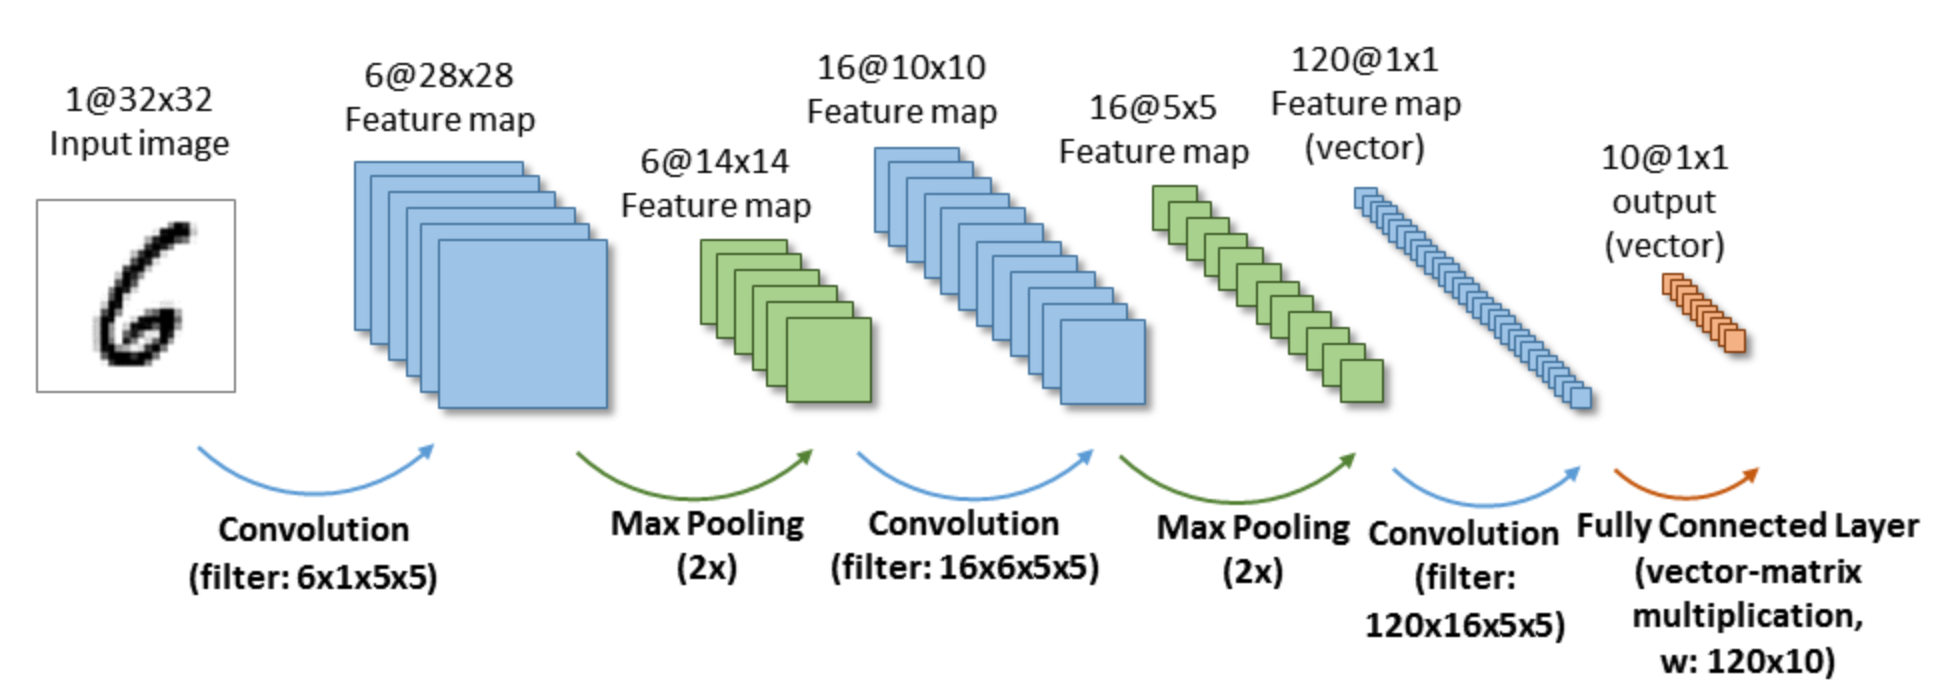
\includegraphics[width=.5\textwidth]{lenet_arch.png}
\caption{lenet architecture highlighting interleaved convolutional and pooling layers}
\end{figure}

\section{Hardware Accelerator Analysis}
Table 2 is a performance analysis of the hardware accelerated implementation. In this part,  components of LeNet were ported to the programmable logic to achieve speed up over the baseline software version.  A detailed account of our design choices for the hardware accelerators are listed below in the Design section. 

\begin{table}[H]
\begin{center}
\caption{Running HLS System on Chip}
\begin{tabular}{lll}
\cline{1-2}
\multicolumn{1}{|l|}{Time Per Image}      & \multicolumn{1}{l|}{DATA} \\ \cline{1-2}
\multicolumn{1}{|l|}{Time For All Images} & \multicolumn{1}{l|}{DATA} \\ \cline{1-2}
\end{tabular}
\end{center}
\end{table} 

Furthermore, Table 3 outlines the resource utilization of the hardware accelerators. The addition of the accelerators did have a reasonable impact on the utilization on the FPGA which can be seen below. The addition of pipelines and loop unrolls significantly increased the LUT and Flip Flop count. 


\begin{table}[H]
\begin{center}
\caption{Resource Usage}
\begin{tabular}{|l|l|}
\cline{1-2}
Flip Flops    & 26170   \\ \cline{1-2}
LUT's         & 21325    \\ \cline{1-2}
BRAM          & 4       \\ \cline{1-2}
DSP           & 12      \\ \cline{1-2}
I/O           & 130     \\ \cline{1-2}
On Chip Power & 2.0009 W \\ \cline{1-2}
\end{tabular}
\end{center}
\end{table}


\subsection{Speedup Over Software Version}
Table 4 is an analysis  of the speed up of the pure software implementation versus the hardware aided implementation. XXXGive reasons into results.

\begin{table}[H]
\begin{center}
\caption{HLS Accelerator Speedup}
\begin{tabular}{lllll}
\cline{1-2}
\multicolumn{1}{|l|}{Speed Up  In Time Per Image}     & \multicolumn{1}{l|}{DATA}  \\ \cline{1-2}
\multicolumn{1}{|l|}{Speed Up In Time For All Images} & \multicolumn{1}{l|}{DATA}  \\ \cline{1-2}
\end{tabular}
\end{center}
\end{table}

\section{Accuracy of Hardware Acceleration}
The hardware accelerated version had an accuracy of 98.39\%. We did not modify the achitecture of the CNN so the accuracy was preserved whether we were running the software or the hardware accellerated version.

\section{System Overview}
The data flow of this MP has a few major parts. First, there is software application running on the embedded ARM core on the board. This is represented by the Zynq Processing System (PS) in Figure 1.  This software application is responsible for loading the SD card data into DRAM as well as maintaining data synchronization with the hardware accelerators. In addition to this the software application was also responsible for XXX in the LeNet algorithm. Not every layer of the neural net was implemented on the programmable logic (PL) side so some layers were implemented in software. The other major component of the system is the hardware accelerators generated by HLS. These accelerators were placed on the programmable logic and were given access to DRAM through the AXI HP ports. The Zynq system sends the accelerators weights, biases, and image data to be processed and then waits for handshake signals from the PL side before it continues with the inference. A description of the accelerators is provided below. 


\section{Hardware Accelerator Description}
\subsection{Accelerated Layers}
In this MP, we accelerated every single layer including the ReLU functions in an attempt to attain the maximum speedup over the software version. We used a combination of HLS Pragmas, Local Buffering, and High Performance DMA AXI ports to move the large quantities of data back and fourth between the PL and PS sides of the SoC. Neural nets are dependent on iterative loops to update the values at every layer. Luckily HLS has pragmas that can take advantage of these loops and parallelize and or pipeline them for more performance. Pretty much every looping construct was unrolled with the \textit{unroll} pragma the the loops were pipelined as well. We also used the local buffering to move data onth the PL fabric so it could be closer to the operational units that will be using the data. Even though the DMA interface is fast buffering the data allowed us to avoid using this interface unless we absolutely had to. Finally we did not want the transfer of data from PS to PL side to be a bottleneck so we used the 

\subsection{Fully Connected Layer}
The fully connected layer has a few different ports to interface the hardware and software. This accelerated block has four AXI High Performace ports. The four ports have DRAM offsets provided by the PS to allow the hardware block to have faster access to DRAM. Our design philosophy was to capitalize on the data locality of the operations in this layer. From this, we made internal buffers that would allow the hardware block to quickly access data instead of waiting on DRAM. There was also opportunity for parallelization in some in the array operations. In our HLS implementation, we used m\_axi port declarations as well as pipeline and loop unrolls. Since we know the size of the loops we were able to get exact loop unroll factors that best fit the sizes of the arrays. We also used a s\_axilite port for control signal passing to the PS. 

\subsection{Convolution1 Layer}
In this layer we also accelerated the \textit{ReLU1}, \textit{max\_pooling2}, and \textit{ReLU2} layers. Again we buffered all inputs and we grouped these operations together into one accelerator to limit the number of times we had to use the DMA interface to synchronize with the PS side. It allows us to avoid overhead of data transfer but it also reduces the testability as there are more points of failure and less visibility into the inner workings of accelerator. We targeted all of the looping constructs with the unrolling and pipelining pragmas. One thing we had to do was change the loop bounds to be static so that the compiler could understand the ranges of the loops.
\begin{mdframed}
\begin{verbatim}

\end{verbatim}
\end{mdframed}


\section{Testing and Verification}



\section{MP Feedback}
Overall this MP was a great learning experience into how HLS can be used to accelerate more complex tasks. A better description into how to work with the SDK functions that interact with the IP's would be helpful for future students. 



\section{Changes to Version of Code}


\section{Difficulties and Bugs}



\section{What We Learned}
In this MP we learned more about the development and control flow of HLS accelerated applications. Working closely with the AXI high performance and AXI lite ports also gave us a better understanding of fast memory interfaces. In addition to this, we also learned more about HLS pragmas and their impact on application performance. 


\section{MP Platform}

\newpage
\begin{verbatim}
//                         Convolution Layer 1
//----------------------------------------------------------------------
int convolution1(float input[1][32][32], float weights[6][1][5][5], float bias[6], float output[6][14][14]) {
#pragma HLS INTERFACE m_axi      depth=1024   port=input   offset=slave bundle=DATA_A
#pragma HLS INTERFACE m_axi      depth=150    port=weights offset=slave bundle=DATA_B
#pragma HLS INTERFACE m_axi      depth=6      port=bias    offset=slave bundle=DATA_C
#pragma HLS INTERFACE m_axi      depth=4704   port=output  offset=slave bundle=DATA_D
#pragma HLS INTERFACE s_axilite  port=return

	/* Local Buffers */
	float c1_i[1][32][32];
	float c1_w[6][1][5][5];
	float c1_b[6];
	float c1_o_a[6][28][28];
	float c1_o_b[6][28][28];
	float c1_o_c[6][14][14];
	float c1_o[6][14][14];

	int k, l;
	int co, h, w, i, m, j, n;
	float sum = 0.0;

     /* Copy to local buffers */
	for(i = 0; i < 32; i++) {
#pragma HLS pipeline II=1
		for(j = 0; j < 32; j++) {
#pragma HLS unroll FACTOR=32
			c1_i[0][i][j] = input[0][i][j];
		}
	}

	for(i = 0; i < 6; i++) {
#pragma HLS pipeline II=1
		for(j = 0; j < 5; j++) {
			for(k = 0; k < 5; k++) {
#pragma HLS unroll FACTOR=5
				c1_w[i][0][j][k] = weights[i][0][j][k];
			}
		}
	}

	for(i = 0; i < 6; i++) {
#pragma HLS unroll FACTOR=6
		c1_b[i] = bias[i];
	}


    /* Convolution 1 */
    for(co = 0; co < 6; co++) {
        for(h = 0; h < 28; h++) {
            for(w = 0; w < 28; w++) {
#pragma HLS unroll FACTOR = 4
                sum = 0.0;
                for(i = h, m = 0; i < (h + 5); i++, m++) {
                    for(j = w, n = 0; j < (w + 5); j++, n++) {
                        sum += c1_w[co][0][m][n] * c1_i[0][i][j];
                    }
                }
                c1_o_a[co][h][w] = sum + c1_b[co];
            }
        }
    }

    /* ReLU 1 */
    for(i = 0; i < 6; i++) {
		for(j = 0; j < 28; j++) {
#pragma HLS pipeline II=1
			for(k = 0; k < 28; k++) {
#pragma HLS unroll FACTOR=28
				c1_o_b[i][j][k] = relu(c1_o_a[i][j][k]);
			}
		}
    }

    float max_value = 0.0;
    int c;

    /* Pooling 2 */
    for(c = 0; c < 6; c++) {
		for(h = 0; h < 14; h++) {
#pragma HLS pipeline II=1
			for(w = 0; w < 14; w++) {
#pragma HLS unroll FACTOR=14
				max_value=-1000000000000.0;
				for(i = h*2; i < h*2+2; i++) {
					for(j = w*2;j < w*2+2; j++) {
						max_value = (max_value > c1_o_b[c][i][j]) ? max_value:c1_o_b[c][i][j];
					}
				}
				c1_o_c[c][h][w] = max_value;
			}
		}
    }

    /* ReLU 2 */
    for(i = 0; i < 6; i++) {
		for(j = 0; j < 14; j++) {
#pragma HLS pipeline II=1
			for(k = 0; k < 14; k++) {
#pragma HLS unroll FACTOR=14
				c1_o[i][j][k] = relu(c1_o_c[i][j][k]);
			}
		}
    }

    /* Copy out of buffer to output */
    for(i = 0; i < 6; i++) {
	    for(j = 0; j < 14; j++) {
#pragma HLS pipeline II=1
             for(k = 0; k < 14; k++) {
#pragma HLS unroll FACTOR=14
                 output[i][j][k] = c1_o[i][j][k];
            }
        }
    }

    return 0;
}
\end{verbatim}



\end{document}
